\documentclass[12pt,a4paper]{article}
\pagestyle{plain}
\usepackage{fullpage}
\usepackage[english]{babel}
\usepackage{enumerate}

%equations
\usepackage[fleqn]{amsmath}
\numberwithin{equation}{section}

%figures
\usepackage[dvips]{graphicx}
\graphicspath{{./images/}}
\numberwithin{figure}{section}

%excercises
\newcounter{Exercise}
\setcounter{Exercise}{1}
\usepackage[dvipsnames]{xcolor}
\usepackage{framed}
\definecolor{shadecolor}{gray}{0.9}
\usepackage{caption}

%tables
\numberwithin{table}{section}

%specials
\usepackage{textcomp} %special (greek) characters as text
\usepackage{pstricks} %more elaborate drawing package
%\usepackage{ifthen} %
%\usepackage{calc} %


%document details
\author{N.G. Schultheiss \\ translated and adapted by K. Schadenberg}
\date{}
\title{Mirrors}


\begin{document}
\maketitle

\section{Introduction}
This module `Mirrors' summarizes and extents your basic knowledge about mirrors. After this module you can proceed with the modules `Lenses' or `Making a parabolic mirror'. When you completed all these modules you should be able to make your own telescope with the help of the module `Making your own telescope' and explain how it works.

\section{Law of Reflection}
The reflection by a smooth shiny surface is governed by the \textbf{Law of Reflection}. This law states that the direction of incoming light (the incident ray) and the direction of outgoing light (the reflected ray) make the same angle with respect to the surface normal, or more briefly the angle of incidence equals the angle of reflection, $\theta_i = \theta_r $. 
\begin{figure}\begin{center}
\setlength{\unitlength}{1mm}
\begin{picture}(100,55)
\put(0,10){\line(1,0){100}}
\put(50,10){\line(0,1){50}}
\thicklines
\put(50,10){\vector(4,1){50}}
\put(50,10){\line(-4,1){50}}
\thinlines
\multiput(1,10)(5,0){20}{\line(1,-1){4}}
\qbezier(35.3003, 14.7781)(37.6333, 25.4432)(48.5412, 24.9887)
\qbezier(64.6997, 14.7781)(62.3667, 25.4432)(51.4588, 24.9887)
\put(44,3){Mirror}
\put(52,60){\rotatebox{-90}{Normal}}
\put(40,27){$\angle$ i}
\put(55,27){$\angle$ r}
\put(2,25){\rotatebox{-14}{Incident ray}}
\put(75,19){\rotatebox{14}{Reflected ray}}
\end{picture}
\caption{Ray diagram showing reflection at a smooth surface.}\label{fig:lawofreflection}
\end{center}\end{figure}

Figure~\ref{fig:lawofreflection} shows how a reflected ray of light can be constructed. The normal is always perpendicular to the surface. The angle of incidence is measured between the ray of light and the normal. Likewise, the angle of reflection is measured between the reflected ray of light and the normal. It is important to measure the angle with the normal, because in doing so we can apply the same method to convex and concave surfaces. 

\begin{shaded}
\textbf{Exercise \theExercise \stepcounter{Exercise}} : Measure the angle of incidence in figure~\ref{fig:lawofreflection}.\end{shaded}

\section{Reflection at spherical mirrors}
In a convex surface, such as the backside of a spoon, you see the world reduced in size. On the inside of the spoon however, you see the world enlarged. This surface is concave. Because a spoon is not a perfect sphere the image of the world is distorted. We will use the law of reflection to predict how light rays are reflected of a convex surface.

\begin{figure}\begin{center}
\setlength{\unitlength}{1mm}
\begin{picture}(100,90)
\put(0,30){\line(1,0){100}}
\thicklines
\put(0,45){\line(1,0){70}}
\put(70,45){\vector(1,4){13}}
\thinlines
\qbezier(83.2, 50.0)(74.9157, 50.0)(69.0579, 44.1421)
\qbezier(69.0579, 44.1421)(63.2, 38.2843)(63.2, 30.0)
\qbezier(63.2, 30.0)(63.2, 21.7157)(69.0579, 15.8579)
\put(81.5,30){\line(-3,4){45}}
\qbezier(55.0014, 45.8088)(54.9015, 52.5995)(60.4183, 56.5602)
\qbezier(61.9446, 57.2035)(66.9954, 61.191)(73.2289, 59.5926)
\put(0,25){Main axis}
\put(75,25){Centre}
\put(81.5,28.5){\line(0,1){3}}
\put(35,15){Reflecting sphere}
\put(0,47){Incident ray}
\put(72,70){\rotatebox{76}{Reflected ray}}
\put(38,90){\rotatebox{-53}{Normal}}
\put(50,55){$\angle$ i}
\put(62,62){$\angle$ r}
\end{picture}
\caption{Ray diagram of reflection at a convex surface.}\label{fig:spherica_reflection}
\end{center}\end{figure}

%\paragraph{} When you look at a reflective sphere you see an image of the world. This image is called a virtual image.

\begin{shaded}
\textbf{Exercise \theExercise \stepcounter{Exercise}} : In figure~\ref{fig:spherica_reflection}
the normal to the reflective surface is already drawn. Explain why the normal goes through the centre of the sphere.\end{shaded}
\begin{shaded}
\textbf{Exercise \theExercise \stepcounter{Exercise}} : A beam of light enters your eye. What shape does this beam need to be for you to see a clear image?\end{shaded}
\begin{shaded}
\textbf{Exercise \theExercise \stepcounter{Exercise}} : When a parallel beam is reflected by a spherical surface the reflected beam will have a certain shape. Describe this shape. Can you see the light source when you look at the reflected beam?\end{shaded}

When we want to magnify images, concave reflecting surfaces can be very useful. The beam path inside a spherical reflective surface is shown in figure~\ref{fig:concave_reflection}.

\begin{figure}\begin{center}
\setlength{\unitlength}{1mm}
\begin{picture}(100,55)
\put(0,30){\line(1,0){70}}
\thicklines
\put(0,45){\line(1,0){56}}
\put(56,45){\vector(1,-4){5}}
\thinlines
\qbezier(63.2, 30.0)(63.2, 38.2843)(57.3421, 44.1421)
\qbezier(57.3421, 44.1421)(51.4843, 50.0)(43.2, 50.0)
\qbezier(43.2, 10.0)(51.4843, 10.0)(57.3421, 15.8579)
\qbezier(57.3421, 15.8579)(63.2, 21.7157)(63.2, 30.0)
\put(44.5,30){\line(3,4){25}}
\qbezier(46.0, 45.0)(46.0, 32.1922)(58.4254, 35.2986)
\put(0,25){Main axis}
\put(35,25){Centre}
\put(44,28.5){\line(0,1){3}}
\put(65,15){Reflecting sphere}
\put(0,47){Incident ray}
\put(65,35){Reflected ray}
\put(55,50){\rotatebox{53}{Normal}}
\put(40,36){$\angle$ i}
\put(50,31){$\angle$ r}
\end{picture}
\caption{Ray diagram of reflection at a concave surface.}\label{fig:concave_reflection}
\end{center}\end{figure}

An image is considered sharp when every point of an object is depicted as a point on the image. If not the points become (large) blobs and the image is unsharp.

\begin{shaded}
\textbf{Exercise \theExercise \stepcounter{Exercise}} : Take a piece of paper and draw a hollow reflecting sphere with a radius of 5.0~cm. Draw a parallel beam with 4 rays placed 1.0, 2.0, 3.0, and 4.0~cm from the main axis. Construct the reflection of these beams using the Law of Reflection. Explain, using your drawing, if a spherical mirror can be used to make sharp images.\end{shaded}

\section{Parabolic and elliptic mirrors}
In the previous section we saw that a spherical mirror, convex or concave, does not produce a neat focal point. To build a telescope, or to otherwise magnify images, we need a differently shaped mirror. In this section we will try and find out what shape is suitable.

We can use the Huygens principle (or Huygens Fresnel principle) to predict how light propagates as a wave. Huygens described light as a wave, not as a particle as his contemporary Newton did. His waves had two important properties: the wave beam and the wave front. The wave beam is similar to the light ray and indicates the direction the light travels in. The wave front is a peak (crest) or trough of the light wave. According to the Huygens principle the next wave front can be found by drawing circles on the wave front with a radius equal to the wave length. The next wave front can be sketched out by drawing the tangent (or tangent curve) to all the circles, see figure \ref{fig:huygens}.

\begin{figure}\begin{center}
\psset{unit=1mm}
\begin{pspicture}*(100,70)
\pscircle(0,35){50}
\pscircle(0,35){60}
\pscircle[linestyle=dotted](41.5,63){10}
\pscircle[linestyle=dotted](46,54){10}
\pscircle[linestyle=dotted](49,45){10}
\pscircle[linestyle=dotted](50,35){10}
\pscircle[linestyle=dotted](49,25){10}
\pscircle[linestyle=dotted](46,16){10}
\pscircle[linestyle=dotted](41.5,7){10}
\put(60,60){Next wave front}
\put(10,60){Wave front}
\put(10,40){Auxiliary circles}
\put(0,35){(Radius = wave length)}
\end{pspicture}
\caption{The Huygens principle.}\label{fig:huygens}
\end{center}\end{figure}

\begin{shaded}
\textbf{Exercise \theExercise \stepcounter{Exercise}} : Look at figure~\ref{fig:huygens}, explain that the previous wave front also touches the drawn circles.\end{shaded}
\begin{shaded}
\textbf{Exercise \theExercise \stepcounter{Exercise}} : Explain why the wave front is always perpendicular to the wave beam.\end{shaded}

A mirror that can be used in a telescope must be able to image a parallel beam of light into a single point. A parallel beam of light according to the Huygens principle can be seen as a sheet of (squared) graph paper. The horizontal lines are the light beam, the vertical lines are the wave fronts. Figure~\ref{fig:plane_wave} shows that a parabolic mirror has a single focal point.

\begin{figure}\begin{center}
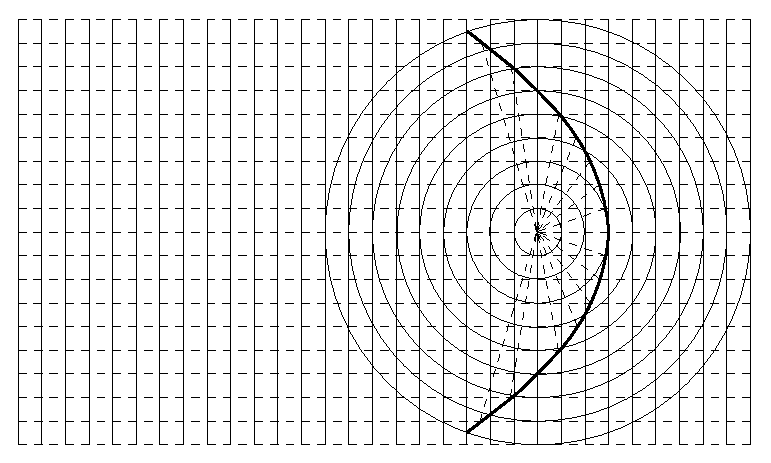
\includegraphics[scale=1.2]{plane_wave.eps}
\caption{A parabolic mirror.}\label{fig:plane_wave}
\end{center}\end{figure}

\begin{shaded}
\textbf{Exercise \theExercise \stepcounter{Exercise}} : Use the Huygens principle to show that the wave fronts become spherical when light converges towards or originates from a single point.\end{shaded}
\begin{shaded}
\textbf{Exercise \theExercise \stepcounter{Exercise}} : Take a look at figure~\ref{fig:plane_wave}. Explain how you can construct the shape of the mirror by connecting the points of intersection of the wave fronts. What happens to the wave front at the surface of the mirror? How many wave lengths does the light travel (from the left) to reach the focal point? Does this distance differ between the different rays?\end{shaded}
\begin{shaded}
\textbf{Exercise \theExercise \stepcounter{Exercise}} : Verify that the mirror in figure~\ref{fig:plane_wave} is parabolic.\end{shaded}

A mirror can be used to image a single point onto a single point. The incident beam of light is in this case divergent instead of parallel. If this divergent beam originated from a single point the wave fronts can be drawn as circles.
\begin{shaded}
\textbf{Exercise \theExercise \stepcounter{Exercise}} : Draw a point of light and a focal point with the appropriate (possible) wave fronts. Construct the mirror needed to image the point of light onto the focal point. Its shape should be elliptical.\end{shaded}

\end{document}
